%% name: Academic Article (English)
%% desc: 論文一式 — 目次・定理・数式・図表フロート・脚注・相互参照・文献
\documentclass{article}
\usepackage{amsmath}
\usepackage{amssymb}
\usepackage{amsthm}
\usepackage{booktabs}
\usepackage{tikz}
\usepackage[a4paper,margin=25mm]{geometry}

\newtheorem{theorem}{Theorem}[section]
\newtheorem{lemma}[theorem]{Lemma}
\newtheorem{definition}[theorem]{Definition}

\title{Your Title Here}
\author{Your Name}

\begin{document}

\maketitle

\tableofcontents

\section{Introduction}
\label{sec:intro}

Start writing here.\footnote{Footnotes are typeset live at the bottom of
the page, rule and all.} Everything in this template --- the table of
contents above, Theorem~\ref{thm:main}, Figure~\ref{fig:example},
Table~\ref{tab:example}, the equations and the citations
\cite{knuth84,lamport94} --- updates as you type.

\section{Mathematics}
\label{sec:math}

Inline math like $\int_0^\infty e^{-x^2}\,dx = \frac{\sqrt{\pi}}{2}$
sits inside the paragraph. Numbered displays carry real counters:

\begin{equation}
  \label{eq:main}
  \nabla \cdot \mathbf{E} = \frac{\rho}{\varepsilon_0}
\end{equation}

\begin{align}
  e^{i\pi} + 1 &= 0, \\
  \sum_{n=1}^{\infty} \frac{1}{n^2} &= \frac{\pi^2}{6}.
\end{align}

Refer to displays with \verb|\eqref|: see~\eqref{eq:main}.

\begin{definition}
  \label{def:example}
  A \emph{resident engine} keeps the full document state alive between
  keystrokes.
\end{definition}

\begin{theorem}
  \label{thm:main}
  A page is patched if and only if its display list hash changes.
\end{theorem}

\begin{proof}
  Immediate from Definition~\ref{def:example}. \qedhere
\end{proof}

\section{Floats}
\label{sec:floats}

Figure~\ref{fig:example} is a real float: it is placed at the top of a
page by the live output routine according to its \texttt{[t]} specifier.

\begin{figure}[t]
\centering
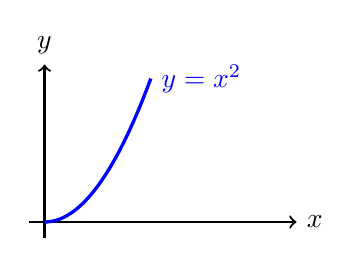
\begin{tikzpicture}[scale=1.0]
  \draw[->, thick] (-0.2,0) -- (3.2,0) node[right] {$x$};
  \draw[->, thick] (0,-0.2) -- (0,2.0) node[above] {$y$};
  \draw[blue, very thick, domain=0:1.35, smooth] plot (\x, {\x*\x})
    node[right] {$y=x^2$};
\end{tikzpicture}
\caption{Edit the coordinates above --- only this block recompiles.}
\label{fig:example}
\end{figure}

\begin{table}[b]
\centering
\begin{tabular}{lrr}
\toprule
Item & Count & Share \\
\midrule
Alpha & 12 & 40\,\% \\
Beta  & 18 & 60\,\% \\
\bottomrule
\end{tabular}
\caption{A bottom float with booktabs rules.}
\label{tab:example}
\end{table}

\section{Conclusion}

As shown in Section~\ref{sec:math}, everything cross-references live.

\begin{thebibliography}{9}
\bibitem{knuth84} Donald E. Knuth. \emph{The \TeX book}.
Addison--Wesley, 1984.
\bibitem{lamport94} Leslie Lamport. \emph{\LaTeX: A Document
Preparation System}. Addison--Wesley, 1994.
\end{thebibliography}

\end{document}
